\bookchapter{Bab 49: Menyiapkan Lingkungan Pengembangan—Android Studio dan Proyek Pertama}

\chapterintro{Ada pepatah: untuk bekerja dengan baik, tajamkan dulu alatmu. Di bab ini kita menyiapkan 'dapurnya': memasang Android Studio, menjalankan emulator, membuat proyek Android pertama dalam hidupmu, lalu membongkar struktur proyeknya sampai benar-benar paham. Setelah lingkungan siap, untuk pertama kalinya kamu akan melihat kode tulisanmu berubah menjadi tombol yang bisa ditekan—momen yang oleh banyak orang diingat seumur hidup.}

\booksection{Memasang Android Studio}

Android Studio adalah lingkungan pengembangan terpadu (IDE) resmi dari Google, gratis, dan fiturnya lengkap: menulis kode, melihat pratinjau tampilan, debugging, sampai mengemas aplikasi semuanya di dalamnya. Pemasangannya empat langkah:

\begin{enumerate}
  \item Buka situs resmi developer.android.com/studio, unduh versi stabil terbaru (per Agustus 2026: versi setelah Narwhal; tersedia untuk Windows/Mac/Linux);
  \item Jalankan berkas pemasangannya, tinggal klik 'Berikutnya' terus—wizard instalasi otomatis menyertakan Android SDK dan komponen emulator;
  \item Saat dijalankan pertama kali, unduh komponen SDK sesuai petunjuk (cukup pakai pilihan bawaan; butuh beberapa menit dan beberapa GB ruang);
  \item Setelah selesai kamu akan melihat halaman selamat datang—selamat, 'dapurnya' sudah terpasang.
\end{enumerate}

\begin{tcbwarn}{Perhatian: Ketahui Persyaratan Perangkat Keras}
Android Studio adalah 'pemakan memori': disarankan RAM minimal 16 GB (8 GB masih bisa jalan, tapi emulatornya agak tersendat saat dibuka), sediakan ruang disk lebih dari 20 GB, dan CPU yang mendukung virtualisasi (aktifkan VT-x/AMD-V di BIOS). Kalau komputermu memang tua, gunakan 'debugging ponsel asli' menggantikan emulator (dibahas di bagian 4 bab ini)—justru lebih lancar.

\end{tcbwarn}

\booksection{Membuat Proyek Pertamamu}

Di halaman selamat datang klik New Project, pilih templat Empty Activity (templat paling bersih untuk pemula), lalu isi tiga hal:

\begin{center}
\begin{tabularx}{\linewidth}{|X|X|X|}
\hline
\textbf{Item Konfigurasi} & \textbf{Isi Dengan Apa} & \textbf{Keterangan} \tabularnewline
\hline
Name & My First App & Nama aplikasi, ditampilkan di layar utama ponsel \tabularnewline
Package name & com.example.myfirstapp & Identitas unik global; kebiasaannya 'domain dibalik', ikuti nilai bawaan dulu \tabularnewline
Minimum SDK & API 26(Android 8.0) & Versi minimum yang didukung, mencakup 95\%+ perangkat \tabularnewline
\hline
\end{tabularx}
\end{center}

\begin{center}\small\color{gray}Tiga hal yang diisi saat membuat proyek\end{center}

Setelah klik Finish, Android Studio akan otomatis mengunduh dependensi dan membangun proyek dengan Gradle (pertama kali perlu menunggu beberapa menit, setelah itu jauh lebih cepat). Begitu build selesai, kamu punya aplikasi yang bisa jalan—walau untuk sekarang hanya menampilkan tulisan 'Hello Android!'.

\begin{tcbinfo}{Tips: Seluk-Beluk Nama Paket}
Nama paket (package name) ibarat 'nomor identitas' aplikasi; tidak boleh ada yang sama di seluruh dunia, dan setelah naik toko tidak bisa diubah lagi. Untuk latihan pribadi, com.example.xxx sudah cukup; produk resmi harus diganti dengan domainmu sendiri yang dibalik (misalnya com.namamu.namaaplikasi). Jangan pernah naik toko dengan com.example—toko akan menolaknya.

\end{tcbinfo}

\booksection{Menjalankannya: Emulator dan Ponsel Asli}

Kode sudah ditulis, sekarang butuh 'ponsel' untuk menjalankannya. Kamu punya dua pilihan:

\booksubsection{Emulator}

Emulator adalah ponsel Android yang divirtualisasi di dalam komputer. Di Android Studio buka Device Manager Create Device, pilih satu perangkat (disarankan seri Pixel) pilih citra sistem (yang ada Google APIs-nya) unduh jalankan. Lalu klik segitiga hijau Run di toolbar; beberapa detik kemudian aplikasimu muncul di layar 'ponsel' itu.

\booksubsection{Debugging Ponsel Asli (Lebih Disarankan)}

Ponsel asli selalu jadi lingkungan uji paling nyata—rasa gesekannya, jaringannya, sensor aslinya, tidak ada yang bisa ditandingi emulator. Debugging dengan ponsel Android asli itu mudah:

\begin{enumerate}
  \item Di ponsel buka [Pengaturan] [Tentang Ponsel], ketuk 'Nomor Versi' 7 kali berturut-turut untuk mengaktifkan 'Opsi Pengembang';
  \item Di [Opsi Pengembang], aktifkan USB Debugging;
  \item Sambungkan ponsel ke komputer dengan kabel data; saat ponsel memunculkan popup, pilih 'Izinkan USB Debugging';
  \item Kembali ke Android Studio, ponselmu akan muncul di daftar perangkat di toolbar, lalu klik Run.
\end{enumerate}

\textbf{Awas Jebakan: Jangan Biarkan USB Debugging Menyala Terus}\par

USB Debugging ibarat membuka 'pintu belakang' bagi komputer. Saat mengisi daya di tempat umum atau menyambung ke komputer yang tidak dipercaya, wajib mematikan USB Debugging agar orang lain tidak bisa membaca datamu lewat jalur itu. Biasakan mematikannya setelah selesai dipakai untuk pengembangan.

\booksection{Bedah Struktur Proyek: Untuk Apa Saja Tiap Berkas}

Pertama kali membuka proyek, pohon berkas di sebelah kiri bisa membuatmu pusing. Tenang, 90\% waktumu dalam pengembangan sehari-hari hanya berurusan dengan beberapa hal berikut:

\begin{center}
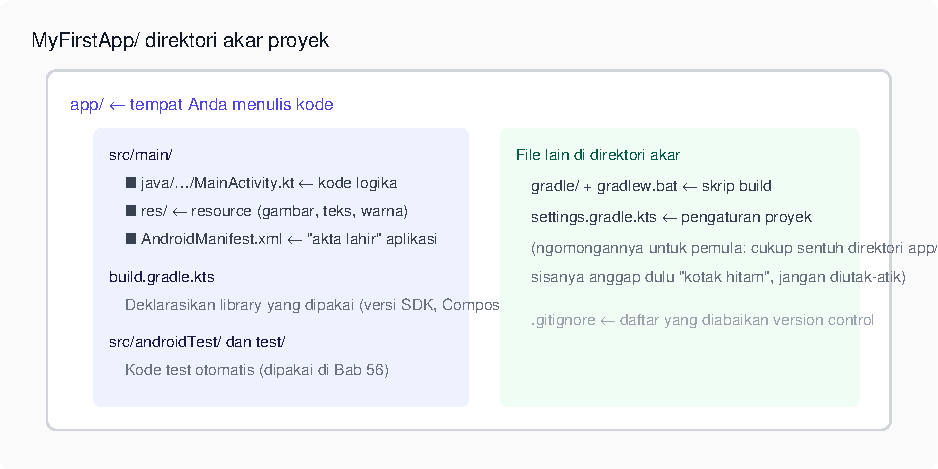
\includegraphics[width=0.92\linewidth]{figures/fig-di-si-shi-jiu-zhang-1}
\\[2pt]\small Gambar 2: Struktur proyek yang wajib dipahami pemula (pegangan: sentuh saja direktori app/)
\end{center}

\begin{itemize}
  \item MainActivity.kt: 'pintu gerbang' aplikasi. Saat pengguna mengetuk ikonnya, inilah yang pertama dibangunkan. Di templat sekarang, ia bertugas menampilkan 'Hello Android!'.
  \item AndroidManifest.xml: 'buku keluarga' aplikasi—menyatakan aplikasi ini bernama apa, ikonnya yang mana, ada halaman apa saja, dan izin apa saja yang dipakai (kamera, lokasi, dst.).
  \item Direktori res/: gudang sumber daya, menyimpan gambar, ikon, teks, warna. Menaruh teks di berkas sumber daya alih-alih menulisnya mati di kode adalah kebiasaan baik pengembangan Android (memudahkan ganti bahasa, ganti tema).
  \item build.gradle.kts: resep build—menyatakan versi minimum yang didukung dan pustaka apa saja yang dipakai (misalnya Compose).
\end{itemize}

\booksection{Coba-Coba: Ganti 'Hello' dengan Namamu}

Buka MainActivity.kt, kamu akan melihat kode yang dihasilkan templat Compose. Temukan baris Text(“Hello Android!”) dan ganti teks di dalam tanda kutip dengan namamu, misalnya Text(“Halo, Budi! Ini aplikasi pertamaku”), lalu tekan Ctrl+R (di Mac Cmd+R) untuk menjalankan ulang. Beberapa detik kemudian namamu tampil di emulator.

\begin{lstlisting}[language=Kotlin]
setContent {
    MyFirstAppTheme {
        Surface(modifier = Modifier.fillMaxSize()) {
            // v Ubah bagian ini menjadi teks Anda sendiri
            Text("Halo, Zhang San! Ini aplikasi pertamaku")
        }
    }
}
\end{lstlisting}

Selamat, kamu baru saja menyelesaikan satu siklus lengkap 'ubah kode kompilasi pasang jalankan'. Siklus inilah rutinitas pengembangan untuk setiap hari ke depan. Sekalian saja coba ubah yang lain: perbesar ukuran huruf, ganti warna—bab berikutnya kita akan belajar dari mana semua 'sihir' itu berasal.

\booksection{Pertolongan Pertama Error Umum: 'Ruang Gawat Darurat' Dua Pekan Pertama Pemula}

Pada tahap penyiapan lingkungan dan build pertama, kemungkinan besar kamu akan menemui tiga error berikut. Tenang, semuanya ada penawarnya:

\begin{center}
\begin{tabularx}{\linewidth}{|X|X|X|}
\hline
\textbf{Gejala Error} & \textbf{Penyebab Umum} & \textbf{Penawarnya} \tabularnewline
\hline
Gradle sync failed / unduhan dependensi lambat & Akses jaringan ke repositori tidak lancar & Konfigurasikan mirror repositori yang lebih cepat untuk Gradle (misalnya mirror maven Alibaba Cloud/Tencent Cloud), cari 'gradle mirror' di internet lalu ikuti petunjuknya \tabularnewline
Komponen SDK kurang & Unduhan SDK terlewat saat instalasi & Lengkapi platform dan alat yang kurang lewat Settings SDK Manager \tabularnewline
Emulator gagal jalan / layar hitam & Virtualisasi belum aktif, citra rusak & Aktifkan VT-x/AMD-V di BIOS; hapus emulator lalu buat ulang; atau langsung pakai debugging ponsel asli \tabularnewline
\hline
\end{tabularx}
\end{center}

\begin{center}\small\color{gray}Tabel pertolongan pertama error lingkungan untuk pemula\end{center}

\begin{tcbinfo}{Tips: Metode Mencari Error}
Baris pertama pesan error paling bernilai—salin persis ke mesin pencari, tambahkan kata kunci 'android studio'. Jangan mencari pertanyaan yang terlalu umum seperti 'kenapa environment saya gagal terpasang'; cari error yang spesifik seperti 'Gradle sync failed: Could not resolve com.android.tools.build'. Pertanyaan yang presisi baru menghasilkan jawaban yang presisi.

\end{tcbinfo}

\begin{tcbpractice}{Praktik: Selesaikan Daftar 'Ritual Peresmian' Pengembangmu}
(1) Pasang Android Studio dan berhasil menjalankan emulator; (2) jalankan aplikasimu sendiri sekali di ponsel asli dan simpan tangkapan layarnya; (3) ubah teks Hello menjadi namamu; (4) arsipkan proyeknya dalam bentuk zip. Selesai empat langkah ini, kamu berhak mengumumkan di media sosial: aku juga pengembang Android sekarang (bukti tangkapan layar).

\end{tcbpractice}

\begin{tcbsummary}{Ringkasan Bab Ini}
\begin{itemize}
  \item Android Studio = IDE resmi gratis; disarankan RAM 16 GB + disk 20 GB + aktifkan virtualisasi
  \item Tiga unsur proyek baru: nama, nama paket (unik global, jangan naik toko dengan com.example), SDK minimum (mulai API 26)
  \item Dua cara menjalankan: emulator (ponsel virtual di komputer) dan ponsel asli (aktifkan USB Debugging, ingat dimatikan setelah pakai)
  \item Pegangan proyek: sentuh saja direktori app/—MainActivity.kt pintu gerbang, Manifest buku keluarga, res/ gudang sumber daya
  \item Rutinitas pengembangan = ubah kode Run lihat hasilnya, berulang-ulang
\end{itemize}

\end{tcbsummary}
